\documentclass[twocolumn]{article}

\usepackage{graphicx}
\usepackage{amsmath}

\title{UW Math 480 Final Project}
\author{Ayla Lampard, Jason Uanon}

\begin{document}
\maketitle
\section{Introduction}

\subsection{Motivation}
\begin{figure*}
    \centering
    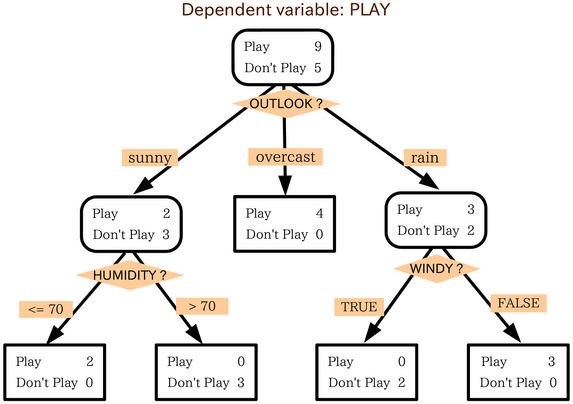
\includegraphics[width=\textwidth]{figs/decision_tree.png}
    \caption{Example of a decision tree}
    \label{decision_tree}
\end{figure*}

Figure~\ref{decision_tree} shows an example of a decision tree.

\subsection{Data}
We will be using the Adult Data Set from the UCI Machine Learning Repository \cite{bache-lichman}. This data is freely-available online and comes from the U.S. Census Bureau from 1994. It contains over 32,000 training instances and 16,000 test instances (although it does contain missing values, denoted with "?". The number of instances with missing values, however, is low enough that we could simply not consider them). 

Using this data, we will create a decision tree that will predict whether a person's income exceeds \$50,000 per year. The data itself contains 14 attributes, which are:

\begin{itemize}
\item age: continuous. 
\item workclass: Private, Self-emp-not-inc, Self-emp-inc, Federal-gov, Local-gov, State-gov, Without-pay, Never-worked. 
\item fnlwgt: continuous. 
\item education: Bachelors, Some-college, 11th, HS-grad, Prof-school, Assoc-acdm, Assoc-voc, 9th, 7th-8th, 12th, Masters, 1st-4th, 10th, Doctorate, 5th-6th, Preschool. 
\item education-num: continuous. 
\item marital-status: Married-civ-spouse, Divorced, Never-married, Separated, Widowed, Married-spouse-absent, Married-AF-spouse. 
\item occupation: Tech-support, Craft-repair, Other-service, Sales, Exec-managerial, Prof-specialty, Handlers-cleaners, Machine-op-inspct, Adm-clerical, Farming-fishing, Transport-moving, Priv-house-serv, Protective-serv, Armed-Forces. 
\item relationship: Wife, Own-child, Husband, Not-in-family, Other-relative, Unmarried. 
\item race: White, Asian-Pac-Islander, Amer-Indian-Eskimo, Other, Black. 
\item sex: Female, Male. 
\item capital-gain: continuous. 
\item capital-loss: continuous. 
\item hours-per-week: continuous. 
\item native-country: United-States, Cambodia, England, Puerto-Rico, Canada, Germany, Outlying-US(Guam-USVI-etc), India, Japan, Greece, South, China, Cuba, Iran, Honduras, Philippines, Italy, Poland, Jamaica, Vietnam, Mexico, Portugal, Ireland, France, Dominican-Republic, Laos, Ecuador, Taiwan, Haiti, Columbia, Hungary, Guatemala, Nicaragua, Scotland, Thailand, Yugoslavia, El-Salvador, Trinadad\&Tobago, Peru, Hong, Holand-Netherlands.
\end{itemize}

\section{Problem Setup}

\subsection{Definitions}

\textbf{Entropy} measures the amount of disorder in a random variable \cite{segaran2007}. Let $X$ be a random variable with $p(x)$ the probability that $X = x$. Mathematically, it can be expressed as 
\begin{align*}
 H(X) &= \sum_{i=1}^{n} p(x_i)\log_{2}\left(\frac{1}{p(x_i)}\right) \\
&= -\sum_{i=1}^{n}p(x_i)\log_{2}\left(p(x_i)\right)
\end{align*}

The \textbf{conditional entropy} of a random variable $X$ (with events $x_i$) conditioned on a random variable $Y$ (with events $y_j$) is
$$ H(X|Y) = -\sum_{i=1}^{n}p(x_i)\sum_{j=1}^{m}p(y_j|x_i)\log_2\left(p(y_j|x_i)\right) $$

The \textbf{information gain} of a random variable $X$ conditioned on a random variable $Y$ is

$$ IG(X) = H(Y) - H(Y|X) $$

\subsection{The Algorithm}

We will be using the ID3 Decision Tree algorithm using information gain as the splitting criteria. 

\begin{itemize}
\item Start from the empty decision tree
\item Select the next best attribute $i$ that maximizes information gain (i.e., maximizing $IG(X_i)$)
\item Recursively build the children of the root node
\end{itemize}

\subsection{Implementation}

We will be using Python 2.7.3 for the implementation of the decision tree algorithms. As part of the project, we will also create a Cython version using Cython 0.15.1 to enhance its performance, and compare the relative speeds of the two implementations.

\begin{thebibliography}{9}

\bibitem{bache-lichman}
Bache, K. and Lichman, M. (2013). \textsl{UCI Machine Learning Repository: Adult Data Set}. [http://archive.ics.uci.edu/ml/datasets/Adult]. Irvine, CA: University of California, School of Information and Computer Science.

\bibitem{segaran2007}
Segaran, Toby. \textsl{Programming Collective Intelligence}. O'Reilly, California, 2007.

\bibitem{mitchell}

\end{thebibliography}

\end{document}
